% !TeX spellcheck = en_GB
\documentclass[main.tex]{subfiles}

\begin{document}
\chapter{Results}
\lhead{Results}
\label{chap:results}

\section{English LUKE Reproduction}%
\label{sec:English LUKE Reproduction}
\begin{table}[H]
	\begin{center}
		\begin{tabular}{l l | c c c c c}
                    Model & Over 5 repetitions & Micro avg. & LOC & PER & ORG & MISC \\
			\hline
                    \multirow{2}{*}{LUKE large}& Mean F1 [\pro]& $94.0$ & $95.0$ & $97.2$ & $93.6$ & $85.2$ \\
                                               & Std. [\pro]& $0.2$  & $0.1$  & $0.1$ & $0.3$ & $1.0$ \\
                    \multirow{2}{*}{LUKE base} & Mean F1 [\pro]& $93.4$ & $94.6$ & $96.8$ & $92.4$ & $84.9$\\
                                               & Std. [\pro]& $0.2$ & $0.2$ & $0.2$ & $0.2$ & $0.7$
		\end{tabular}
	\end{center}
	\caption{
        Observed English LUKE results over five repetitions of fine-tuning and evaluating LUKE on CoNLL-2003 for each model size.
        }
	\label{tab:lukeF1s}
\end{table}
Yamada et al. report micro avg. F1 scores of 94.3\pro\ and 93.3\pro\ for LUKE large and base, respectively \cite{yamada2020luke}.
In both cases, the reported scores are within two standard deviations on observed F1 scores, estimated on training repetition.
This is expected and we conclude that the reproduction was successful.
However, the variability of fine-tuning is also highlighted here and will be discussed in Section~\ref{sec:fine-tuning-exp}.
% However, it also highlights the variability of the fine-tuning.
% With margins between top-performing models being as small as they are \cite{pwc21ner}, whoever can claim SOTA may well come down to who got the luckiest seeds.
% This could be mitigated by reporting the mean of several fine-tunings, but Yamada et al. at least do not mention having done multiple fine-tunings.

\section{Pretraining of DaLUKE}
\label{sec:Pretraining of DaLUKE}
\begin{figure}[H]
    \centering
    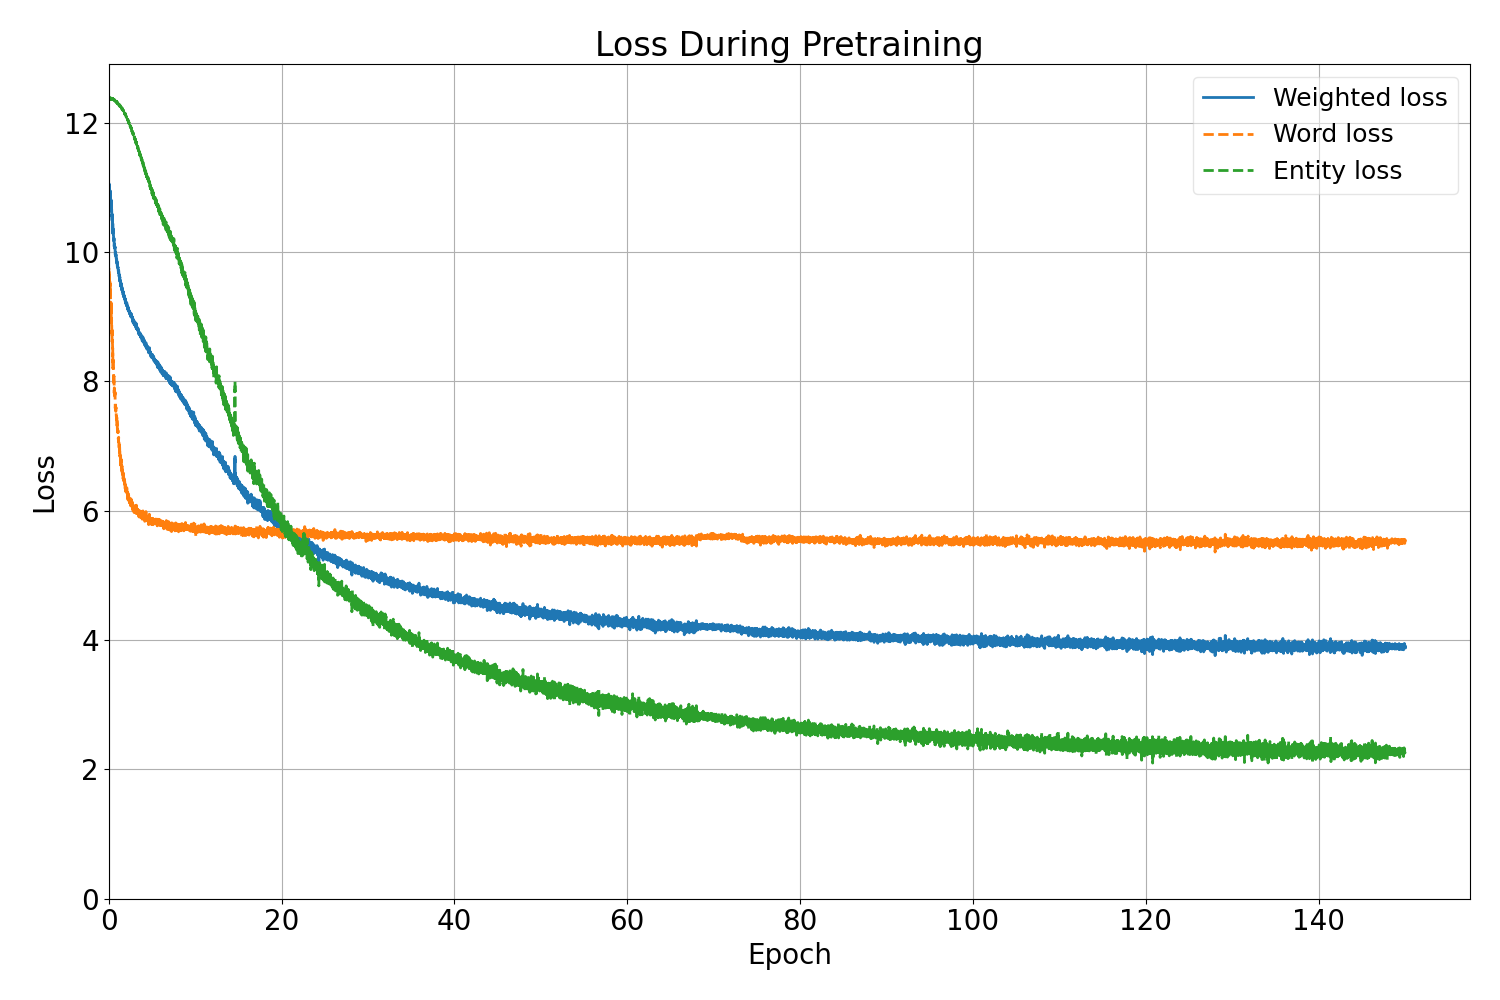
\includegraphics[width=.7\textwidth]{loss}
    \caption{
    Cross entropy loss throughout pretraining for both masking tasks as well as effective (weighted) loss, which is the average of the two.
    The loss on the entity masking (green) seems to drive close to all development in the average loss (blue) after the first few epochs.
    }
    \label{fig:loss}
\end{figure}\noindent

\begin{figure}[H]
    \centering
    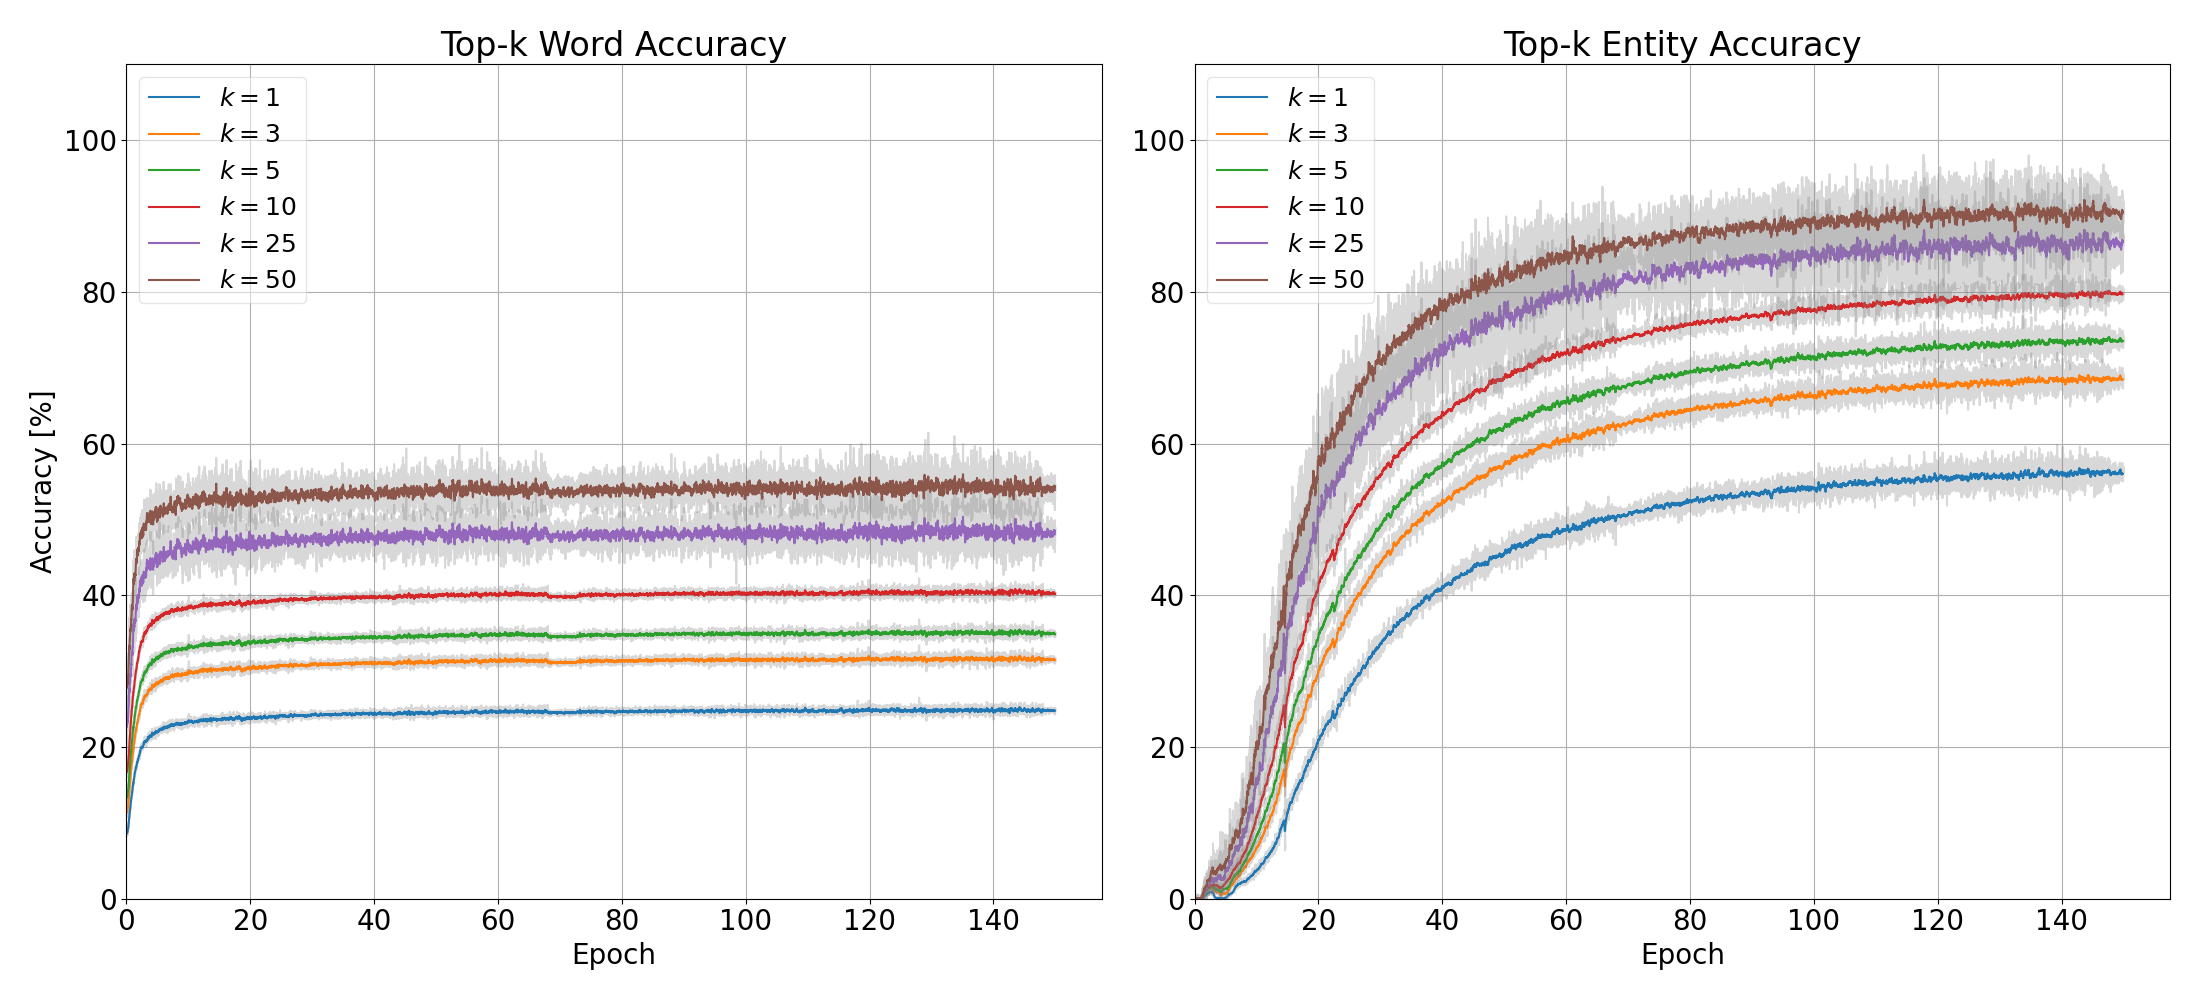
\includegraphics[width=\textwidth]{pretrain-acc}
    \caption{
    Masked subwords and masked entity accuracy throughout pretraining.
    The curves are smoothed with a rolling average.
    The frequency of exact correct word guesses quickly rests at 20-25\pro\ while the new task of entity masking starts from 0 and takes time to learn.
    }
    \label{fig:pretrain-acc}
\end{figure}\noindent
The loss shown on Figure \ref{fig:loss} mirrors the accuracy with masked subword loss converging quickly, after which falling entity loss becomes the driving factor behind the falling total loss.
The masked subwords and masked entity accuracies are shown on Figure \ref{fig:pretrain-acc}.
The former converges quickly, achieving close to top accuracy in less than a tenth of the full training time, while the latter keeps improving throughout the training.
That the masked language modeling performance from BERT is quickly maximized is, however, perhaps not surprising, as many of the relevant weights are initialized from an already trained model which has been pretrained on the exact same task.

\begin{table}[H]
    \centering
    \begin{tabular}{l|rrrrrr}
        Top $k$ accuracy [\pro] & $k=1$  & $k=3$ & $k=5$ & $k=10$ & $k=25$ & $k=50$\\\hline
        Masked words            & 24.82       & 31.54      & 34.96      & 40.27       & 48.15       & 54.02      \\
        Masked entities         & 56.17       & 68.58      & 73.58      & 79.78       & 86.36       & 90.27
    \end{tabular}
    \caption{
        The main pretrained model performance in the last of 150 epochs.
        We note that the model has learned to guess masked entities consistently as the correct entity very often is one of within top 50 guesses.
    }
    \label{tab:mainpre}
\end{table}\noindent
\section{Danish Named Entity Recognition}%
\label{sec:nerres}

\subsection{Main Benchmark: Our Results and Reproduction}
              % precision    recall  f1-score   support

 % ┆   ┆   LOC     0.8365    0.9062    0.8700        96
 % ┆   ┆  MISC     0.7652    0.7273    0.7458       121
 % ┆   ┆   ORG     0.7956    0.6770    0.7315       161
 % ┆   ┆   PER     0.9441    0.9389    0.9415       180

 % ┆ micro avg     0.8467    0.8118    0.8289       558
 % ┆ macro avg     0.8354    0.8124    0.8222       558
% weighted avg     0.8440    0.8118    0.8262       558

              % precision    recall  f1-score   support

 % ┆   ┆   LOC     0.8365    0.9062    0.8700        96
 % ┆   ┆   ORG     0.7956    0.6770    0.7315       161
 % ┆   ┆   PER     0.9441    0.9389    0.9415       180

 % ┆ micro avg     0.8690    0.8352    0.8518       437
 % ┆ macro avg     0.8588    0.8407    0.8477       437
% weighted avg     0.8658    0.8352    0.8484       437
\begin{table}[H]
        \footnotesize
        \begin{center}
                \begin{tabular}{l l | c c c c | c c c c}
                    \multirow{2}{*}{Model name} & \multirow{2}{*}{Trained on} & \multicolumn{4}{c|}{Micro Avg. [\pro]} & \multicolumn{4}{c}{Class F1 [\pro]}\\
                                      &           & F1            & Prec.         & Rec.          & F1 {\tiny\textdiscount MISC} & LOC            & PER            & ORG            & MISC \\\hline
                        DaLUKE        & DaNE      & 82.9          & 84.7          & 81.2          & 85.2                        & \textbf{87.0} & \textbf{94.2} & 73.2          & 74.6 \\\hline
                        DaNLP da-BERT & DaNE      & --            & --            & --            & 84.0                        & 83.9          & 92.8          & 73.0          & -- \\
                        NERDA m-BERT  & DaNE      & 79.2          & 82.1          & 76.5          & 81.7                        & 83.5          & 92.6          & 66.9          & 70.3 \\
                        NERDA Ælæctra & DaNE      & 70.6          & 76.1          & 65.8          & 74.5                        & 77.3          & 86.9          & 56.2          & 56.4 \\
                        DaCy medium   & DaNE      & 78.3          & 78.3          & 78.3          & 80.5                        & 84.0          & 90.4          & 66.2          & 70.1 \\
                        DaCy large    & DaNE      & \textbf{84.9} & \textbf{86.2} & \textbf{83.7} & \textbf{86.9}               & 85.3          & \textbf{94.2} & \textbf{79.0} & \textbf{78.1} \\
                        DaNLP spaCy   & DaNE      & 73.8          & 76.1          & 71.5          & 75.7                        & 76.0          & 87.8          & 59.6          & 66.1 \\
                        DaNLP Flair   & DaNE      & --            & --            & --            & 81.8                        & 84.8          & 93.2          & 63.0          & -- \\
                        Polyglot      & Wikipedia & --            & --            & --            & 64.2                        & 65.0          & 78.7          & 39.3          & -- \\
                        daner         & ITU CDT   & --            & --            & --            & 56.5                        & 59.4          & 70.4          & 28.3          & --
                \end{tabular}
        \end{center}
        \caption{
            F1\pro-scores of Danish NER models of the DaNE testing dataset consisting of 565 sentences.
        Missing numbers is due to a number of models not being trained on the MISC annotations.
        We see the transformer based models dominate the scores, spearheaded by the large implementation of DaCy.
        }
        \label{tab:DaNE}
\end{table}\noindent

\begin{figure}[H]
    \centering
    \begin{minipage}{.49\textwidth}
        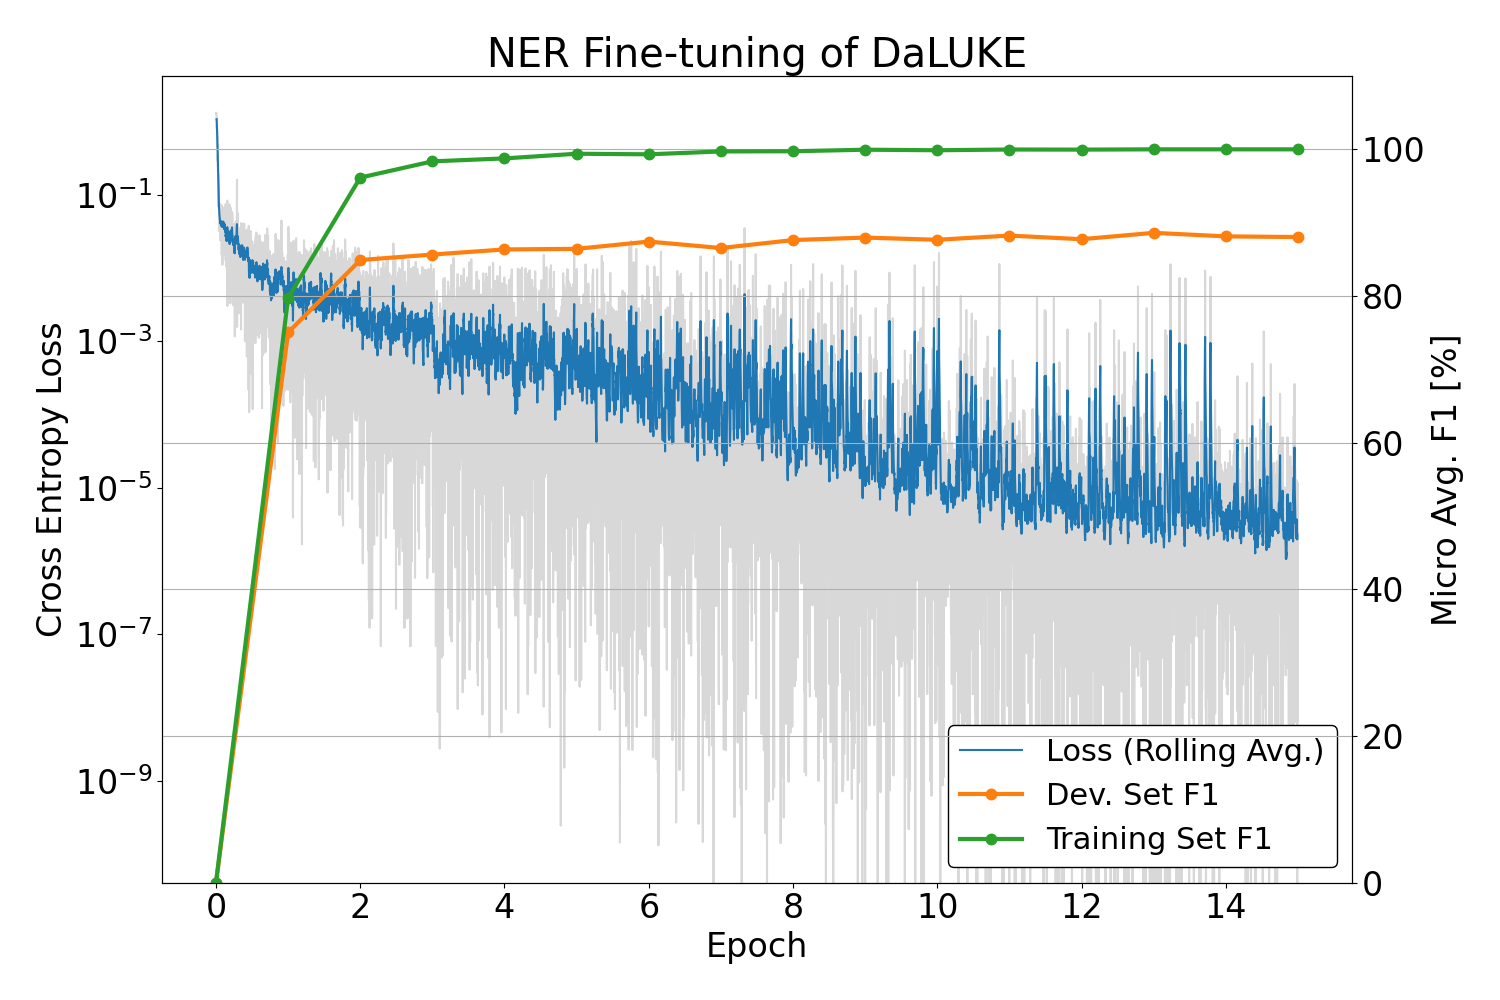
\includegraphics[width=\textwidth]{loss-fine}
    \end{minipage}\hfill
    \begin{minipage}{.49\textwidth}
        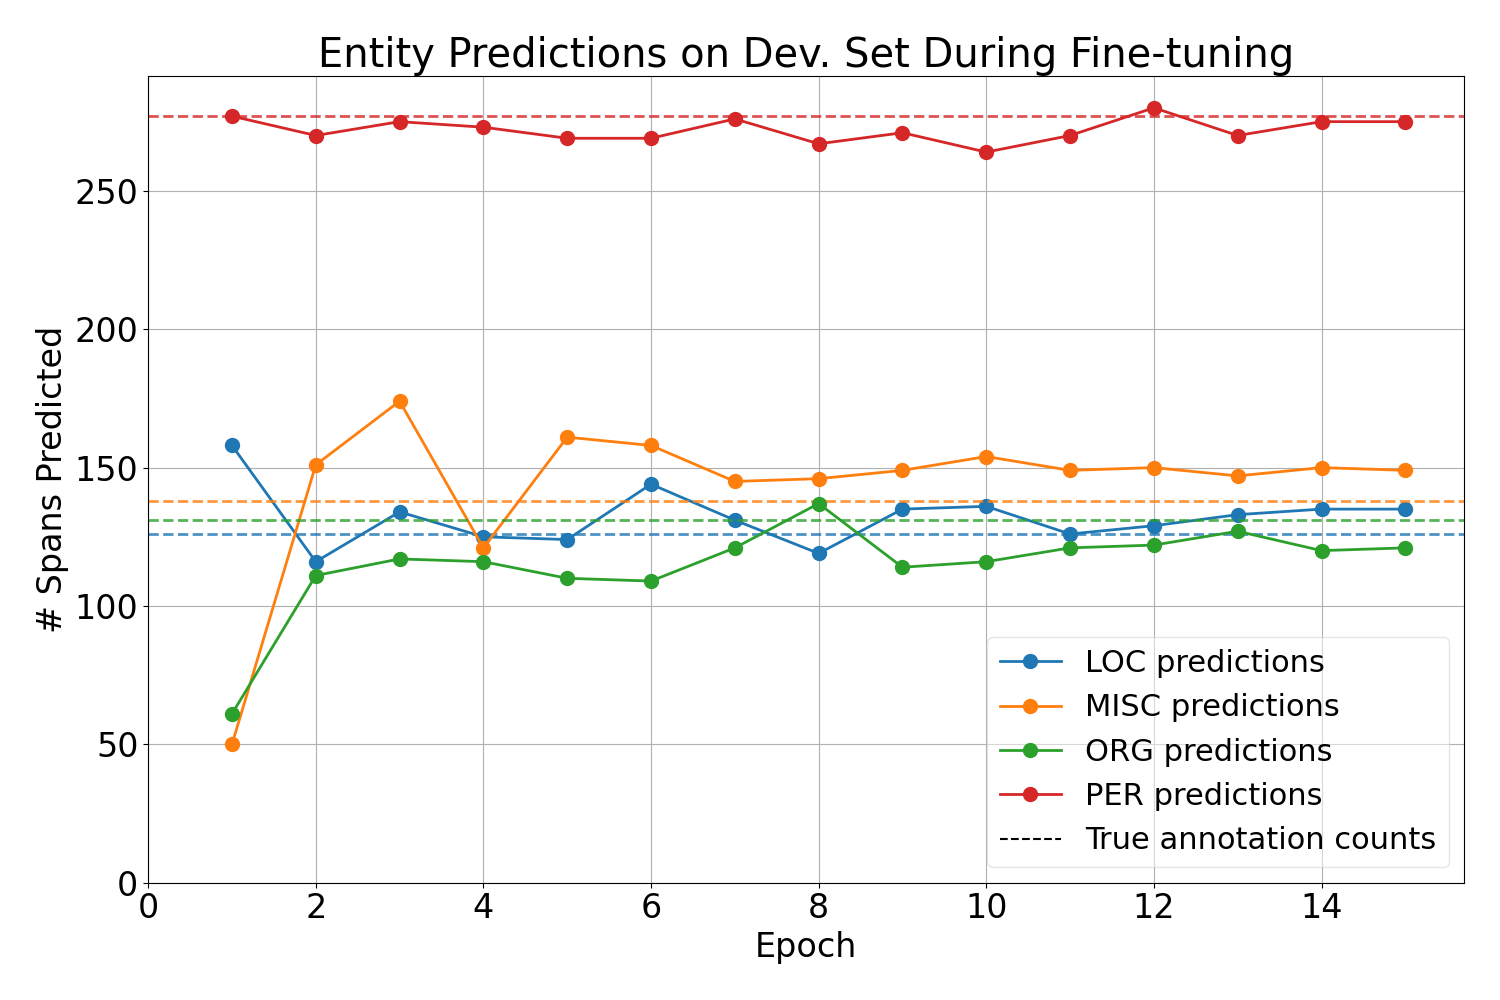
\includegraphics[width=\textwidth]{dev-dists}
    \end{minipage}
    \caption{
        To the left, the development of loss and accuracy on the DaNE training and dev. sets.
        Almost all learning happens in the first few epochs, hinting that the pretrained model already holds much of the language knowledge used for NER.
        To the right, the number of predictions of each class on the dev. set is shown along with the actual number of each class where MISC and ORG initially are under-predicted.
    }
    \label{fig:main-fine-tune}
\end{figure}\noindent
We conclude, when comparing with the June 2021 DaNLP NER table\footnotemark \cite{danlp2021}, the results of all NER algorithms previously reported on DaNE are successfully reproduced with most being exactly correct and a few varying within a percentage point.
\footnotetext{
    Table is available at \url{github.com/alexandrainst/danlp/blob/master/docs/docs/tasks/ner.md} and was compared at the 27/6, 2021 at commit SHA \code{584d5c7}.
}
DaLUKE fails to achieve SOTA on DaNE, being beaten only by DaCy large.
However, it does beat da-BERT on which it is based, indicating that the extra pretraining and entity understanding indeed has added some knowledge to the model.
Interestingly, DaLUKE still manages to pull off a first place in the LOC category and ties DaCy large in PER, while falling behind in both ORG and MISC.
Future analysis of DaLUKE should examine whether this is due to bias in the Wikipedia pretraining dataset.

Ultimately, DaLUKE still performs at a high level and shows its promise for entity modeling.

\subsection{Additional Datasets}
              % precision    recall  f1-score   support

 % ┆   ┆   LOC     0.8298    0.8041    0.8168        97
 % ┆   ┆  MISC     0.0849    0.3000    0.1324        30
 % ┆   ┆   ORG     0.4710    0.6915    0.5603        94
 % ┆   ┆   PER     0.8994    0.9527    0.9253       169

 % ┆ micro avg     0.6054    0.8026    0.6902       390
 % ┆ macro avg     0.5713    0.6871    0.6087       390
% weighted avg     0.7162    0.8026    0.7493       390
              % precision    recall  f1-score   support

 % ┆   ┆   LOC     0.8298    0.8041    0.8168        97
 % ┆   ┆   ORG     0.4710    0.6915    0.5603        94
 % ┆   ┆   PER     0.8994    0.9527    0.9253       169

 % ┆ micro avg     0.7397    0.8444    0.7886       360
 % ┆ macro avg     0.7334    0.8161    0.7675       360
% weighted avg     0.7688    0.8444    0.8008       360
\begin{table}[H]
        \footnotesize
        \begin{center}
                \begin{tabular}{l l | c c c c | c c c c}
                    \multirow{2}{*}{Model name} & \multirow{2}{*}{Trained on} & \multicolumn{4}{c|}{Micro Avg. [\pro]} & \multicolumn{4}{c}{Class F1 [\pro]}\\
                                      &                & F1             & Prec.        & Rec.           & F1 {\tiny\textdiscount MISC} & LOC & PER & ORG & MISC \\\hline
                        DaLUKE        & DaNE           & \textbf{69.0} & \textbf{60.5} & 80.3          & 78.9         & \textbf{81.7} & \textbf{92.5}   & 56.0          & 13.2 \\\hline
                        DaNLP da-BERT & DaNE           & --            & --            & --            & \textbf{79.2}& 78.6          & 93.4            & \textbf{56.9} & -- \\
                        NERDA m-BERT  & DaNE           & 66.4          & 58.1          & 77.4          & 76.6         & 76.3          & 92.1            & 52.5          & 12.4 \\
                        NERDA Ælæctra & DaNE           & 66.3          & 60.0          & 74.1          & 76.1         & 74.9          & 90.3            & 53.0          & 13.2 \\
                        DaCy medium   & DaNE           & 65.6          & 55.7          & 79.7          & 75.0         & 76.1          & 92.1            & 48.7          & 12.6 \\
                        DaCy large    & DaNE           & 68.5          & 58.9          & \textbf{81.8} & 79.0         & 79.0          & \textbf{92.5}   & 58.0          & \textbf{15.5} \\
                        DaNLP spaCy   & DaNE           & 64.1          & 55.9          & 75.1          & 72.7         & 72.7          & 88.3            & 46.5          & 12.3 \\
                        DaNLP Flair   & DaNE           & --            & --            & --            & 76.2         & 80.2          & 94.4            & 36.1          & -- \\
                        Polyglot      & Wikipedia      & --            & --            & --            & 64.1         & 69.7          & 78.4            & 24.7          & -- \\
                        daner         & ITU CDT        & --            & --            & --            & 59.8         & 58.2          & 73.6            & 26.1          & --
                \end{tabular}
        \end{center}
        \caption{
        F1\pro\ scores of Danish NER models of the Plank test set consisting of 565 sentences.
        }
        \label{tab:Plank}
\end{table}

              % precision    recall  f1-score   support

 % ┆   ┆   LOC     0.7626    0.7085    0.7346      5242
 % ┆   ┆   ORG     0.6497    0.3347    0.4418      4078
 % ┆   ┆   PER     0.7239    0.7757    0.7489      4378

 % ┆ micro avg     0.7267    0.6187    0.6684     13698
 % ┆ macro avg     0.7121    0.6063    0.6418     13698
% weighted avg     0.7166    0.6187    0.6520     13698
\begin{table}[H]
        \footnotesize
        \begin{center}
                \begin{tabular}{l l | c c c | c c c }
                    \multirow{2}{*}{Model name} & \multirow{2}{*}{Trained on} & \multicolumn{3}{c|}{Micro Avg. [\pro]} & \multicolumn{3}{c}{Class F1 [\pro]}\\
                        & & F1 & Prec. & Rec. & LOC & PER & ORG \\
                        \hline
                        DaLUKE          & DaNE      & \textbf{66.8} & \textbf{72.7} & 61.9          & 73.5          & 74.9          & 44.2 \\\hline
                        DaNLP da-BERT   & DaNE      & 65.7          & 68.6          & 63.2          & 72.1          & 74.5          & 40.1 \\
                        NERDA m-BERT    & DaNE      & 63.4          & 61.3          & 65.7          & 70.7          & 76.9          & 48.4 \\
                        NERDA Ælæctra   & DaNE      & 48.7          & 48.3          & 49.0          & 56.6          & 69.9          & 24.0 \\
                        DaCy medium     & DaNE      & 60.1          & 58.4          & 61.8          & 70.7          & 73.7          & 39.3 \\
                        DaCy large      & DaNE      & 64.6          & 62.2          & \textbf{67.1} & \textbf{74.1} & \textbf{77.2} & \textbf{49.8} \\
                        DaNLP spaCy     & DaNE      & 59.6          & 58.5          & 60.6          & 68.7          & 71.6          & 38.8 \\
                        DaNLP Flair     & DaNE      & 65.0          & 70.7          & 60.2          & 70.1          & 74.4          & 43.7 \\
                        Polyglot        & Wikipedia & 62.9          & 66.3          & 58.2          & 72.4          & 69.2          & 35.3 \\
                        daner           & ITU CDT   & 46.6          & 51.5          & 42.5          & 56.2          & 54.5          & 14.8
                \end{tabular}
        \end{center}
        \caption{F1\pro\ scores of Danish NER models of the WikiANN test set consisting of 10,000 sentences.}
        \label{tab:WikiANN}
\end{table}
When fine-tuned on DaNE, DaLUKE achieves achieves SOTA both when evaluated on the Plank and WikiANN test sets, though only when including MISC and by a small margin on Plank.
This is unexpected given that DaLUKE is beaten on the DaNE test set.
It may indicate a better generalization ability, which, if true, is indeed a desirable property.
However, less exciting reasons for this behaviour may well be more likely.
With Plank, the difference is miniscule and may simply be explained by variance.
As shown in Section \ref{sec:English LUKE Reproduction} and \ref{sec:luke-stability}, this affects LUKE on CoNLL-2003 and DaLUKE on DaNE.
The performance discrepancy on WikiANN may be even less exciting:
That DaLUKE is pretrained directly on similar, annotated Wikipedia data, violating the principle that the training and test sets should be disjoint.

\end{document}
